% \subsection{Systèmes actuels de SLU}
%         \begin{enumerate}
%             \item (Ré-)Entrainement de modèles de langue masqué (BERT-based) $\implies$ Besoin de beaucoup de données annotées 
%             \item Prompting de \textbf{ChatGPT} avec peu ou pas d'exemples~\cite{He2023, Zhu2024}.  $\implies$ Besoin de moins/pas de données annotées.
%         \end{enumerate}
% %   pour les tâches de Slot Filling et de classification d'intention, tantôt de manière jointe entre intention et slots ou de manière séparée~\cite{He2023}.


% \subsection{Croissement des Tâches : Intent \& SF}
% \begin{columns}
% \begin{column}{0.5\textwidth}
    
%     \begin{enumerate}
%         \item Résolution la tâche d'intent par le LLM $\implies$ \texttt{Intention Silver}
%         \item 
%         \begin{itemize}
%             \item Injection de l'\texttt{Intention Silver} dans le prompt SF 
%             \item Selection de slots candidats selon \texttt{Intention Silver} 
%         \end{itemize}
%         $\implies$ Prompt SF \emph{différents} pour chaque intention.
%     \end{enumerate}

% \end{column}
% \begin{column}{0.5\textwidth}  %%<--- here
% \begin{figure}
%     \centering
%     \includegraphics[width=0.7\textwidth]{assets/CroissementDesTachesSLU_Prompting.pdf}
%     \caption{Croissement des Tâches}
% \end{figure}
% \end{column}
% \end{columns}
% 
% \subsection{Exemple d'intents/slots (SNIPS)}

% Enoncé : "Add I Will Survive to my playlist"\\
% Intention: \texttt{AddToPlaylist}

% \begin{tcolorbox}
% \begin{itemize}
% \tightlist
% \item \texttt{PlayMusic}\\ \textbf{Candidate slots} : artist, album, service, music\_item, track, year, playlist, genre.
% \item \textcolor{BrickRed}{\texttt{\textbf{AddToPlaylist}}}\\ 
% \textbf{Candidate slots} : entity\_name, playlist, artist, music\_item.
% \item $\cdots$
% \end{itemize}
% \end{tcolorbox}
% 
% \subsection{Exemple de prompt (SNIPS)}
%     \centering
% \label{prompt:user}
% \resizebox{0.9\textwidth}{!}{
% \begin{tcolorbox}[title=Prompt Utilisateur, text width=\textwidth]
% The intent of the sentence is "\textcolor{BrickRed}{\textbf{AddToPlaylist}}".\\
% Annotate the sentence with slots (extract the relevant information), given the following slots and their descriptions:\\
% \textbf{entity\_name}: entity name\\
% \textbf{artist}: artist\\
% \textbf{playlist}: playlist\\
% \textbf{music\_item}: music item\\
% \\
% ---\\
% User: "add count von cosels obsession to jazzy romance"\\
% Info: \textbf{entity\_name}: count von cosels obsession; \textbf{playlist}: jazzy romance\\
% ---\\
% User: "add the track bg knocc out to the rapcaviar playlist"\\
% Info: \textbf{music\_item}: track; \textbf{artist}: bg knocc out; \textbf{playlist}: rapcaviar\\
% ---\\
% User: "Add I Will Survive to my playlist"\\
% Info:\\
% \end{tcolorbox}
% }
% 
% \subsection{Délimitation des intentions de SNIPS et MEDIA}
% \centering
% % Pour SNIPS : 7 intentions qui ont toutes entre 2 et 14 concepts. Pour
% % MEDIA : 11 intentions qui ont toutes entre 4 et 72 concepts.
% Fonctionne bien quand les intentions délimitent bien les concepts.
% \begin{columns}[t]
%         \begin{column}{0.5\textwidth}
%             \begin{table}
%             \resizebox{\textwidth}{!}{
%                 \begin{tabular}{lrr}
%                     \toprule
%                     Intent & Nbr concepts & Fréq (\%) \\
%                     \midrule
%                     SearchCreativeWork & 2 & 9.52 \\
%                     \textbf{AddToPlaylist} & 5 & 14.55 \\
%                     RateBook & 7 & 20.80 \\
%                     SearchScreeningEvent & 7 & 12.03 \\
%                     GetWeather & 9 & 12.80 \\
%                     PlayMusic & 9 & 12.35 \\
%                     BookRestaurant & 14 & 17.92 \\
%                     \bottomrule
%                 \end{tabular}
%                 }
%             \caption{SNIPS Dataset}\label{tbl-first}

%             \end{table}
            
%         \end{column}
%         \begin{column}{0.5\textwidth}
%             \begin{table}
%             \resizebox{\textwidth}{!}{
%                 \begin{tabular}{lrr}
%                 \toprule
%                 intent & Nbr concepts & Fréq (\%) \\
%                 \midrule
%                 marqueur\_discursif & 4 & 0.039 \\
%                 annulation & 17 & 0.21 \\
%                 reponse\_indecise & 24 & 0.23 \\
%                 remercier & 28 & 0.85 \\
%                 incomprehension & 43 & 0.83 \\
%                 modification & 43 & 1.38 \\
%                 saluer & 51 & 2.33 \\
%                 reponse\_negative & 59 & 6.21 \\
%                 reponse\_affirmative & 61 & 18.02 \\
%                 renseignements & 63 & 14.12 \\
%                 reservation & 72 & 55.75 \\
%                 \bottomrule
%                 \end{tabular}
%             }
%             \caption{MEDIA Dataset}\label{tbl-second}
%             \end{table}
%         \end{column}
%     \end{columns}
% 
% \subsection{SNIPS: Peu de partage de concept entre intentions}

% \#Concepts liés à 1 unique intention : 8+4+5+5+4+2=28

% \begin{figure}
%     \centering
%     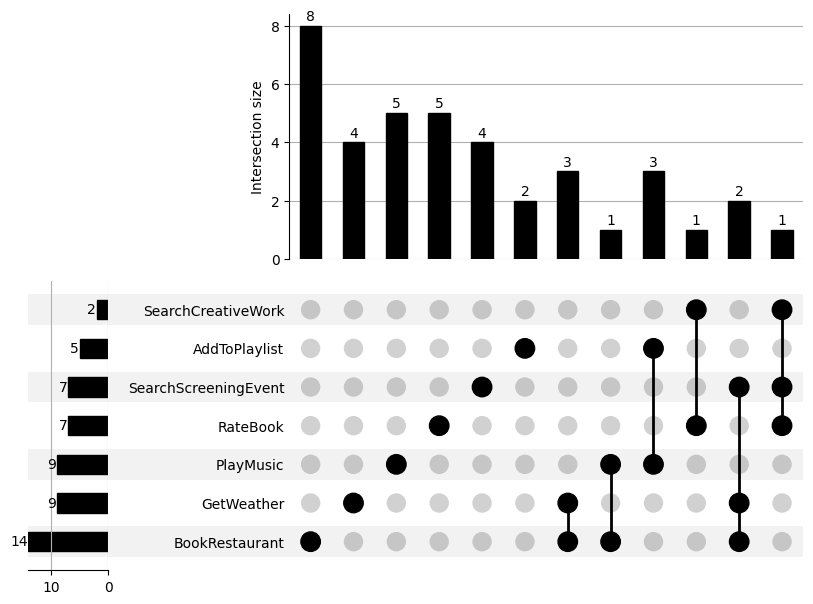
\includegraphics[height=0.45\linewidth]{assets/SNIPS_Labels.png}
%     \caption{Recoupements des Intentions: SNIPS}
%     \label{fig:SNIPS-labels}
% \end{figure}

% 

% \subsection{MEDIA: Beaucoup de partage de concept entre intentions}

% \begin{itemize}
%     \tightlist
%     \item 3 concepts liés à 1 unique intention : reservation $\rightleftharpoons$ localisation-region, personne-nomDeFamille, hotel-etat
%     \item 1 concepts liés à toutes les intentions: reponse
% \end{itemize}

% \begin{figure}
%     \centering
%     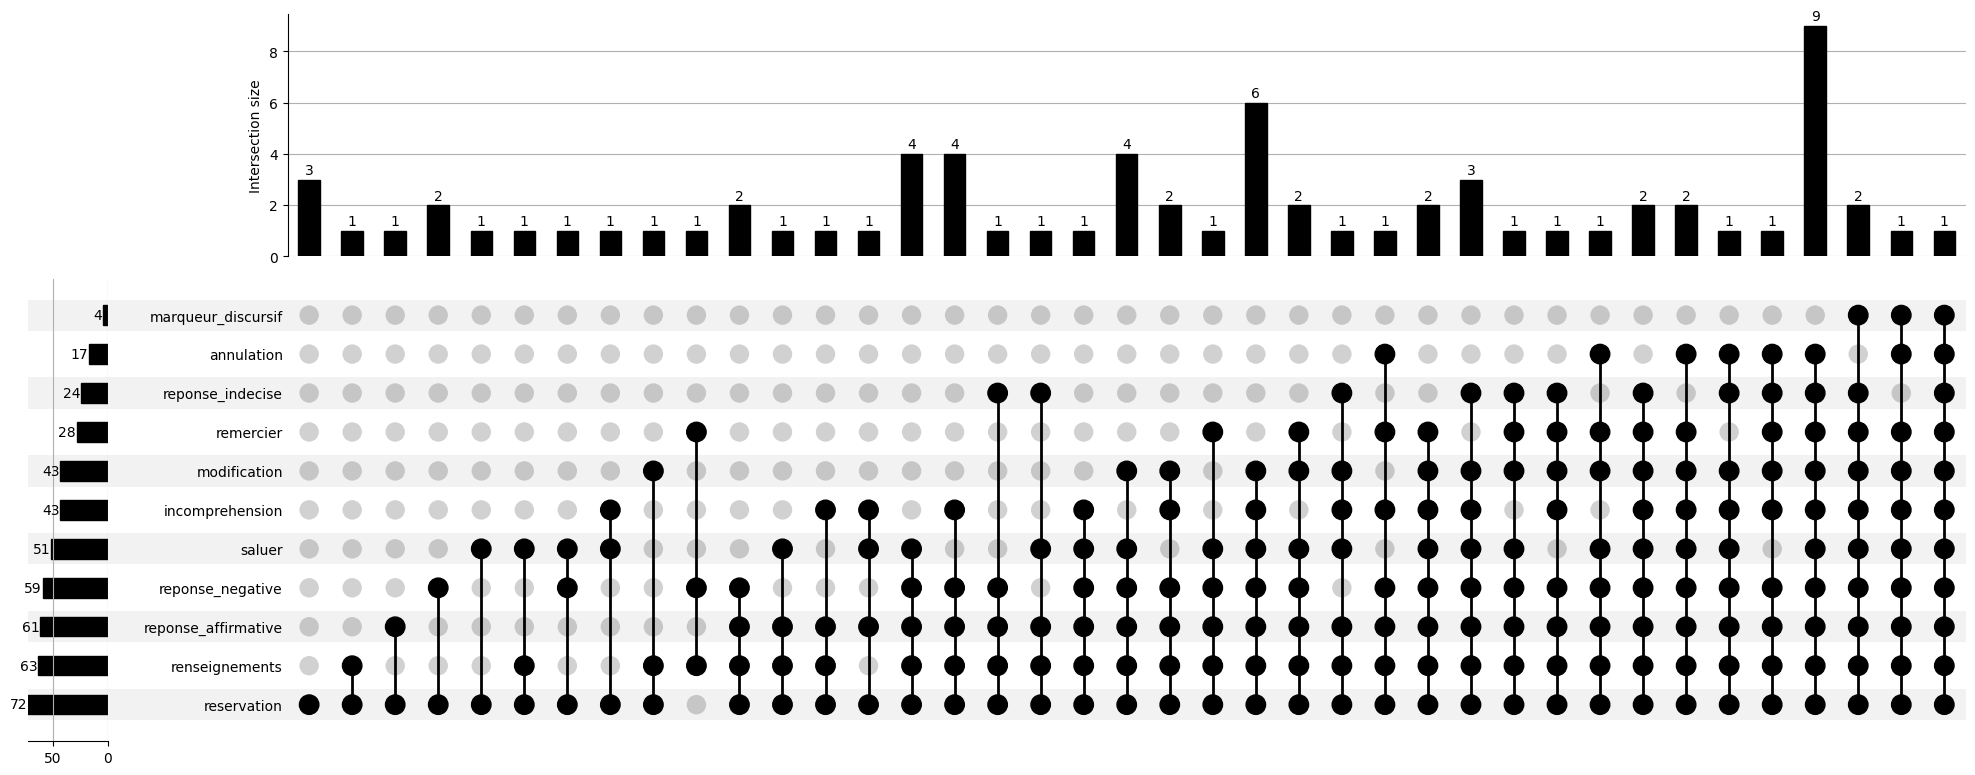
\includegraphics[width=0.95\linewidth]{assets/MEDIA_Labels.png}
%     \caption{Recoupements des Intentions: MEDIA}
%     \label{fig:MEDIA-labels}
% \end{figure}
% 
% \subsection{Ce qui soulèvent des questions...}
%         \begin{enumerate}
%             \item Quelle strategie quand les intents ne séparent pas bien les concepts entre eux ? (MEDIA)
%             \item Comment cette stratégies se comparent-elle à l'état de l'art ? 
%             \begin{itemize}
%                 \item Performance absolue ?
%                 \item Longueur de prompt et coût de calcul ?
%                 \item Pourquoi une autre méthode fonctionnerais ?
%                 \item Est-ce qu'il existe un nombre d'exemples optimal pour le prompt ?
%                 \item Quelles performance attendre dans différentes langues que l'anglais ?
%             \end{itemize}
%         \end{enumerate}
% 

% \subsection{Quelle strategie quand les intents ne séparent pas bien les concepts entre eux ? }
%   Proposition: Remplacer une sélection \emph{basée sur l'intent} par une sélection \emph{basée sur l'utterance} directement $\implies$ Approches par Recherche d'Information. 
%   \begin{figure}
%     \centering
%     \includestandalone[width=\linewidth]{assets/Diagram_IR} % without the `.tex` extension
%   \end{figure}  
% 
% \subsection{Matériel Expérimental}
% \begin{itemize}
%     \item Model: \texttt{NousResearch/Hermes-3-Llama-3.1-8B}
%     \item Système RI : BM25, ColBERT \& SPLADE
%     \item Datasets: 
%         \begin{table}[]
%             \centering
%             \begin{tabular}{c|ccc}
%                  Dataset & Langue & \# Utterances &\# Slots\\
%                  \hline
%                  SNIPS & EN &  &\\
%                  ATIS & EN & &\\
%                  SLURP & EN &  &\\
%                  MASSIVE & FR, ES, PT, DE&  &\\
%                  MultiATIS++ & FR, ES, PT, DE &  &\\
%                  MEDIA & FR &  &\\
%             \end{tabular}
%             \caption{Datasets Utilisés}
%             \label{tab:my_label}
%         \end{table}
% \end{itemize}
% 
% \subsection{Matériel Expérimental (Prompt et condition de génération)}\label{prompt:system}
%     \centering
% \begin{itemize}
%     \item Prompt Final : Concatenation du Sytem Prompt ~(slide \ref{prompt:system}) $\oplus$ Prompt Utilisateur~(slide \ref{prompt:user})\\
%     \item Génération de 256 tokens en greedy decoding.
% \end{itemize}

% \resizebox{\textwidth}{!}{
% \begin{tcolorbox}[title=System Prompt, text width=\textwidth]
% % <|begin\_of\_text|><|im\_start|>system\\
% You are an expert annotator for slot filling tasks.\\
% You must capture all possible slot-value pairs.\\
% You need to output the annotations in the form of 'Slot1=VALUE1;Slot2=VALUE2;...'.\\
% You must only output the slot annotations.
% \end{tcolorbox}
% }
% 
% \subsection{Baselines \& Métriques}

% \begin{itemize}
%     \item Methode Selection (Tirage de $K$ examples) 
%     \begin{enumerate}
%         \item Random-Based Selection : Tirage aléatoire dans la base d'exemples
%         \item Intent-Based Selection \cite{Mirza2024,qin2024cropromptcrosstaskinteractiveprompting}: Tirage aléatoire dans la base d'exemples \textbf{parmis les exemples de même intent que l'utterance}.
%     \end{enumerate}
%     \item Metriques
%     \begin{enumerate}
%         \item Score F1
%         \item Concept Error Rate
%     \end{enumerate}
% \end{itemize}
% 


% \section{Résultats}
% \subsection{Performance absolue \& Longueur de prompt}
% \subsection{Performance absolue: Full Dataset - EN}

% \begin{figure}
%     \centering
%     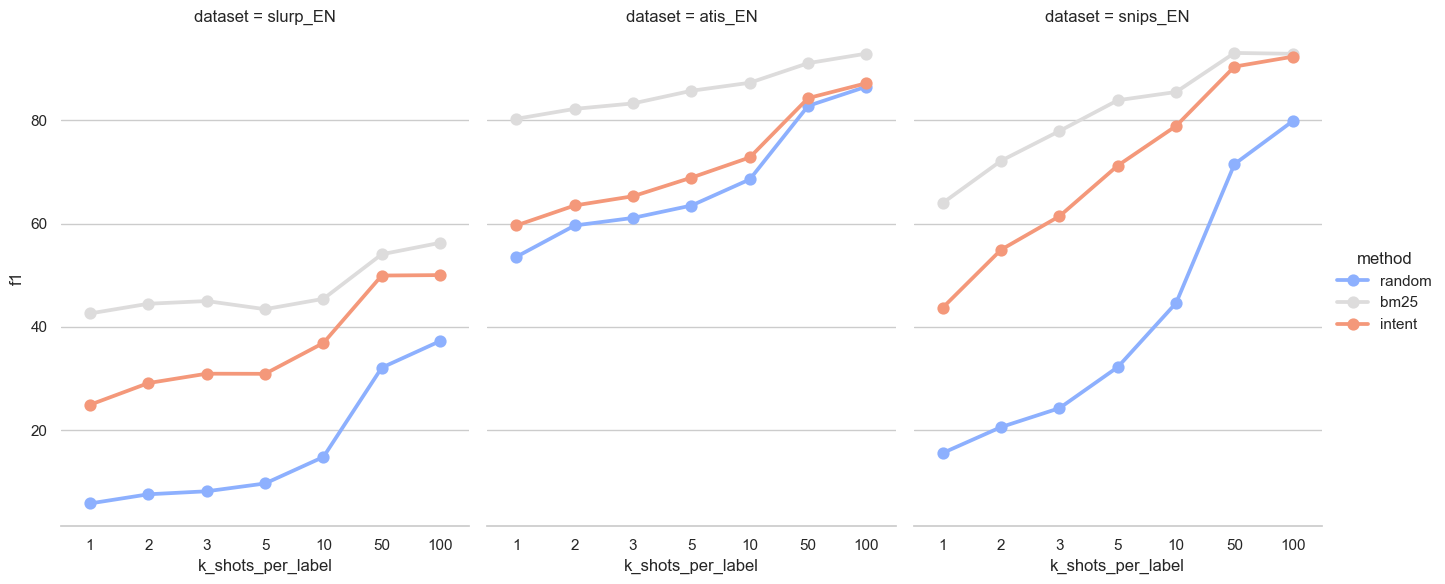
\includegraphics[width=\linewidth]{assets/Results/bm25_outperforming_EN.png}
%     \caption{F1 Score pour K exemples dans le prompt par méthode}
%     \label{fig:BM25-EN}
% \end{figure}
% 
% \subsection{Longueur de prompt et coût de calcul}    
% \begin{figure}
%     \centering
%     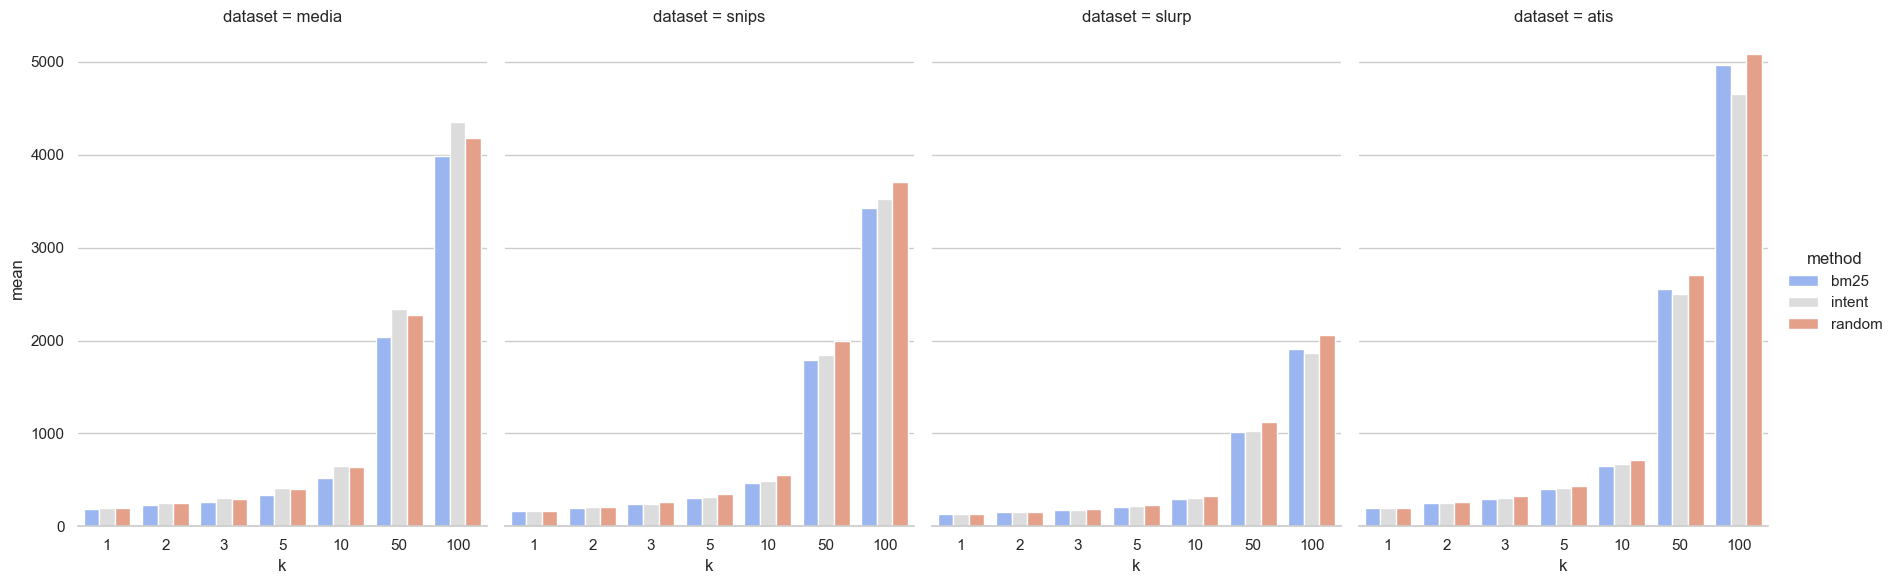
\includegraphics[width=\linewidth]{assets/Results/Taille_prompts.png}
%     \caption{Tailles des prompts pour K exemples par méthode}
%     \label{fig:Prompt_Length}
% \end{figure}
% 
% \subsection{Longueur de prompt et coût de calcul}    
% \centering
% \begin{columns}[t]
%         \begin{column}{0.4\textwidth}
%             \begin{table}
%             \resizebox{0.6\textwidth}{!}{
%                 \begin{tabular}{llr}
%                 \toprule
%                 dataset & method & mean \\
%                 \midrule
%                 \multirow[c]{3}{*}{atis} & bm25 & 1330 \\
%                  & \textbf{intent} & \textbf{1286} \\
%                  & random & 1389 \\
%                 \cline{1-3}
%                 \multirow[c]{3}{*}{media} & \textbf{bm25} & \textbf{1081} \\
%                  & intent & 1217 \\
%                  & random & 1176 \\
%                 \cline{1-3}
%                 \multirow[c]{3}{*}{slurp} & \textbf{bm25} & \textbf{556} \\
%                  & \textbf{intent} & \textbf{556} \\
%                  & random & 602 \\
%                 \cline{1-3}
%                 \multirow[c]{3}{*}{snips} & \textbf{bm25} & \textbf{940} \\
%                  & intent & 969 \\
%                  & random & 1034 \\
%                 \bottomrule
%                 \end{tabular}
%                 }
%             \caption{Prompt length for each dataset}\label{table:prompt_size}
%             \end{table}
%         \end{column}
%         \begin{column}{0.6\textwidth}
%             \begin{itemize}
%                 \item Random-Selection : crée des prompts en moyenne plus long que les deux autres. 
%                 \item Intent-Selection \& BM25-Selection : crée des prompts des longeurs similaires.
%             \end{itemize}
%         \end{column}
%     \end{columns}
% 
% \subsection{Est-ce qu’il existe un nombre d’exemples optimal pour le prompt ?}

% Optimal : Meilleur performance / Longueur de prompt

% 
% \section{Quelles performance attendre dans différentes langues que l’anglais ?}

% \subsection{Performance absolue: Full Dataset - FR}
% \begin{figure}
%     \centering
%     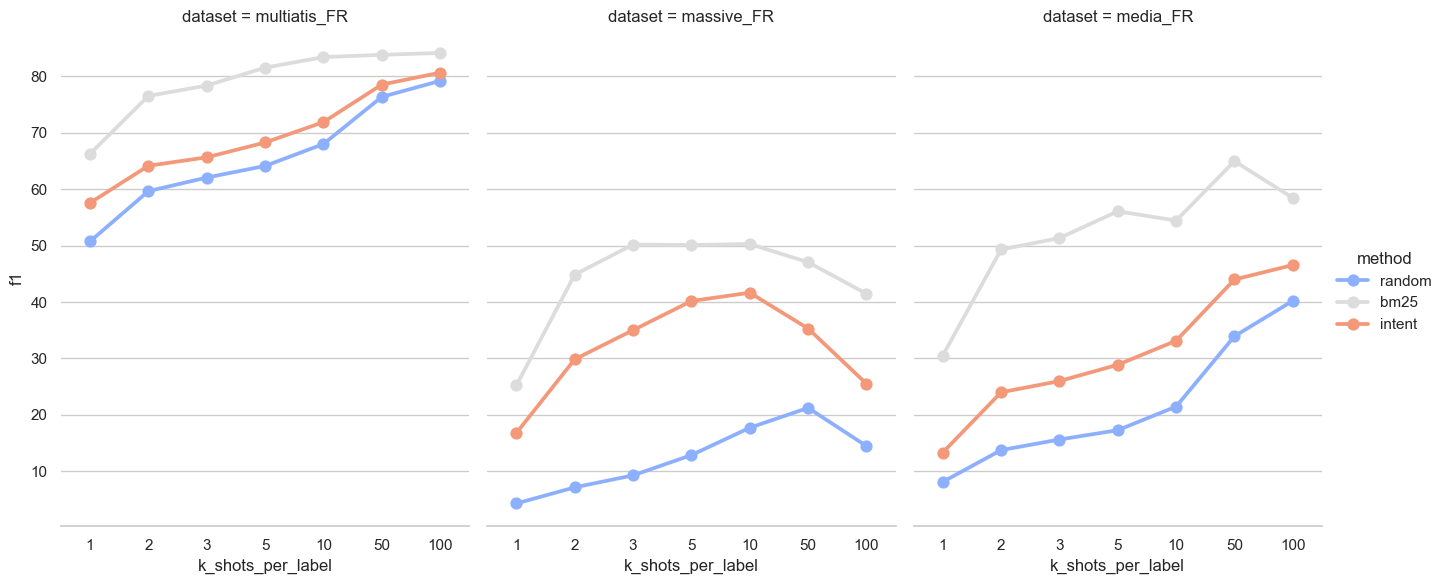
\includegraphics[width=\linewidth]{assets/Results/bm25_outperforming_FR.png}
%     \caption{F1 Score pour K exemples dans le prompt par méthode}
%     \label{fig:BM25-FR}
% \end{figure}
% 
% \subsection{Performance absolue: Full Dataset - Autres}
% \begin{figure}
%     \centering
%     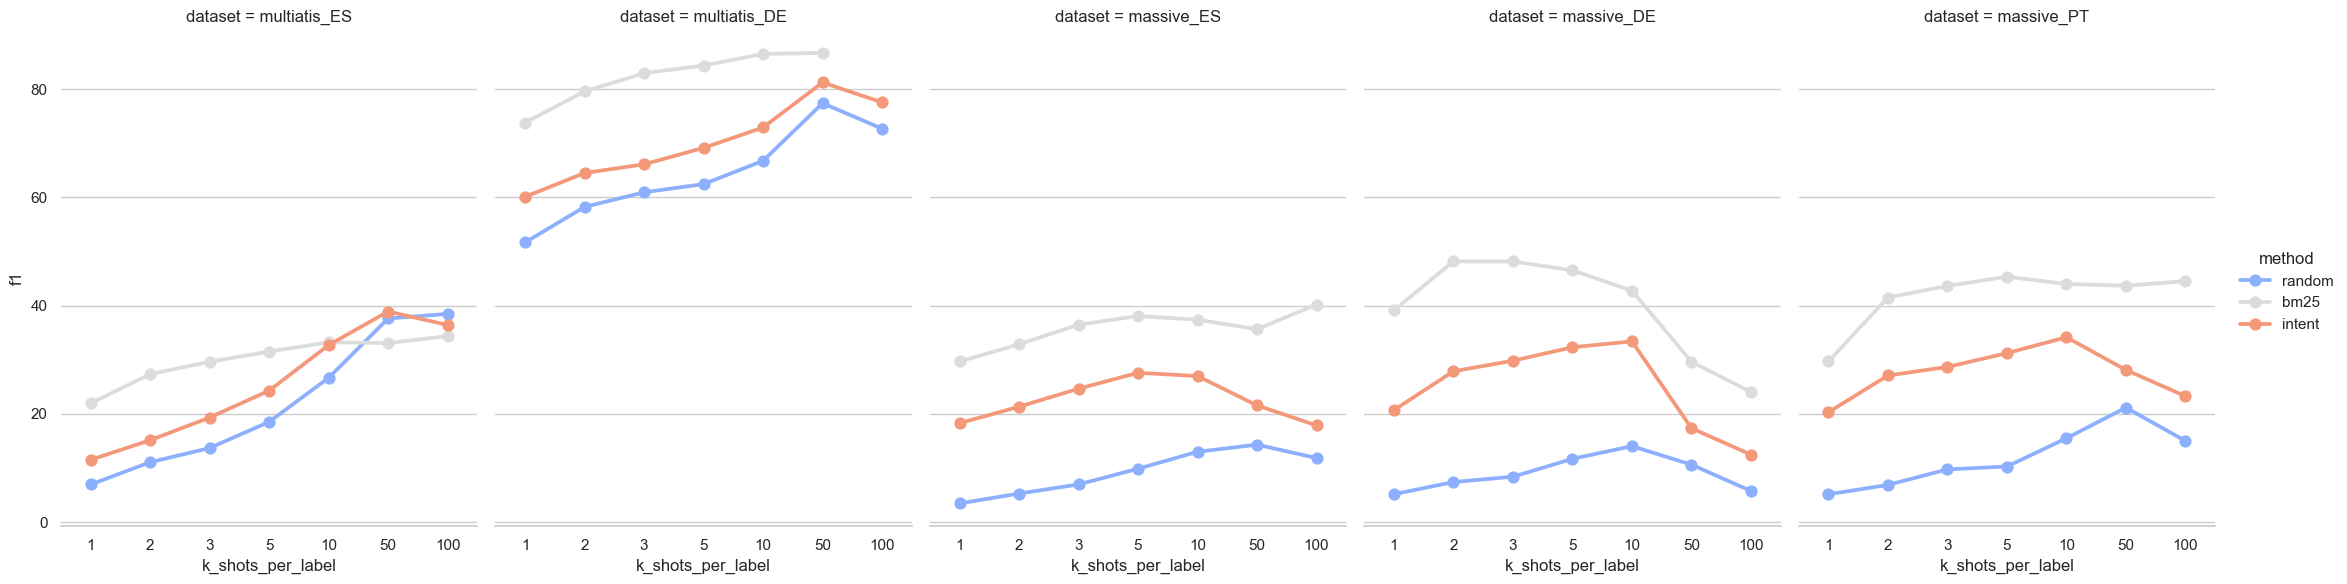
\includegraphics[width=\linewidth]{assets/Results/bm25_outperforming_OTHERS.png}
%     \caption{F1 Score pour K exemples dans le prompt par méthode}
%     \label{fig:BM25-OTHERS}
% \end{figure}
% 

% \section{To Do \& Next Step}

% \subsection{To Do \& Next Step}
% \begin{enumerate}
%     \item Se comparer avec Illuminer~\cite{Mirza2024} correctement :\\ 
%         Faire tourner l'experience sur MASSIVE et SNIPS avec 
%     \begin{itemize}
%         \item Model : \texttt{WizardLMTeam/WizardLM-13B-V1.2} 
%     \end{itemize}
%     \item Ajouter Analyse Qualitative des erreurs dans les générations.
%     \item Lancer expérience de réduction de la base d'exemples.\\ 
%     \item Créer et lancer expérience de création iterative de la base d'exemples.
% \end{enumerate}    
% 
% % \maketitle


% % \begin{abstract}
% % The understanding of spoken language (SLU) has made significant progress thanks to prompt-based language models. However, constructing effective prompts remains a challenge, particularly regarding specificity and length. This study proposes a new approach to selecting examples for SLU prompts using information retrieval (IR) techniques. We hypothesize that this method will outperform traditional approaches, such as intent-based selection, in terms of performance and computational efficiency. 
% % Our study compares Lexical and semantic IR methods across various SLU datasets, including SNIPS, ATIS, and MEDIA. We explore the impact of the number of selected examples and evaluate the efficiency of partially using the training dataset. Additionally, we examine the robustness of our approach in a multilingual context using the MultiAtis++ and Massive datasets.
% % % (BM25, ColBERT, SPLADE)
% % The results show that our IR-based selection method significantly improves performance in terms of Slot F1 Score and Concept Error Rate while reducing the length of prompts. We identify an optimal number of examples to include, which varies depending on the dataset's characteristics. The approach also demonstrates consistent efficiency across different languages. This study contributes to the optimization of prompts for SLU, offering a solution to the dual challenge of specificity and length. Our findings have significant implications for improving the efficiency and accuracy of SLU systems in various linguistic and application contexts.
% % \end{abstract}

% % \section{Introduction}

% % Spoken Language Understanding (SLU) is a crucial area of artificial intelligence aimed at enabling machines to interpret and respond to human language in a precise and contextual manner. At the heart of this field, SLU focuses specifically on interpreting spoken input, a particularly complex challenge due to the nuances of human speech.

% % Recently, the advent of Large Language Models (LLMs) has revolutionized the field of Natural Language Understanding (NLU), delivering unprecedented performance across various linguistic tasks. These models, trained on vast corpora of text, have demonstrated a remarkable ability to understand and generate natural language. However, their effectiveness heavily depends on the quality of the prompts used to guide them in specific tasks.

% % In this context, prompt optimization has become a crucial research focus. Prompts serve as specific instructions given to LLMs to direct their processing towards a particular task. For SLU, these prompts need to be precise enough to capture the subtleties of spoken language while remaining general enough to accommodate the diversity of oral expressions.

% % \section{Approche proposée: Sélection d'exemples par recherche d'information}

% % Ici inserer un graphique et un algo.

% % \begin{algorithm}
% % \caption{Incorporating Retrieved Examples into Prompt}
% % \begin{algorithmic}[1]
% % \Require Current $x$, Retrieval System $R$, Maximum Examples $K$, Prompt Template $T$
% % \Ensure Final Prompt $P$

% % \State $E \gets R(x,K)$ \Comment{Retrieve up to K examples relevant to the query}
% % \State $P \gets T$ \Comment{Initialize prompt with template}

% % \For{each example $e$ in $E$}
% %     \State $formatted\_e \gets$ FormatExample($e$) \Comment{Format the example as needed}
% %     \State $P \gets P \oplus$ formatted\_e \Comment{Append formatted example to prompt}
% % \EndFor

% % \State $P \gets P \oplus x$ \Comment{Append the original query to the prompt}

% % \Return $P$
% % \end{algorithmic}
% % \end{algorithm}

% % \section{Méthodologie expérimentale}

% % \subsection{Datasets}

% % \begin{table}[!h]
% % \centering
% % \resizebox{\columnwidth}{!}{

% % \begin{tabular}{lcccccccc}
% %     \toprule
% %     Dataset & \multicolumn{2}{c}{ATIS} & \multicolumn{2}{c}{MEDIA} & \multicolumn{2}{c}{SLURP} & \multicolumn{2}{c}{SNIPS} \\
% %     \cmidrule(lr){2-3} \cmidrule(lr){4-5} \cmidrule(lr){6-7} \cmidrule(lr){8-9} 
% %     & Train & Test & Train & Test & Train & Test & Train & Test \\
% %     \midrule
% %         \textbf{Nb. utterances}  & 4978 & 893 & 13712 & 3767  & 11514 & 2974 & 13084 & 700 \\
% %         %\textbf{Mean Size of utterances} & 127.64  & 35.72 & 253.93 & 80.15 & 397.03 & 114.38 & 484.59 & 33.33 \\
% %         \textbf{Nb. Concepts}  & 80 & 70 & 73 & 71  & 56 & 54  & 40 & 70  \\
% %     \bottomrule
% %   \end{tabular}
% % }

% % \caption{The number and the average size of the utterances,  and the number of concepts, in Train and Test sets for ATIS, MEDIA, SLURP and SNIPS}
% % \label{tab:shortstats}
% % \end{table}

% % Our study focuses on four well-known SLU tasks (details in table~\ref{tab:shortstats}): 
% % %ATIS, SNIPS, SLURP, and MEDIA:
% % \begin{enumerate}
% %     \tightlist
% %     \item ATIS~\cite{hemphill-etal-1990-atis}: 
% %     The ATIS (Airline Travel Information System) dataset contains queries about airline travel information in English.
% %     \item SNIPS~\cite{coucke2018snips}: 
% %     SNIPS benchmark is an English-only dataset from the SNIPS personal assistant.
% %     \item SLURP~\cite{bastianelli-etal-2020-slurp}:
% %     The SLURP (Spoken Language Understanding Resource Package) Dataset is an English-only dataset simulating single-turn interactions between users and a voice-controlled assistant.
% %     \item MEDIA~\cite{bonneaumaynard05_interspeech, alavoine:hal-04523286}: 
% %     The dataset is about hotel reservations and information. MEDIA corpus is available in a \textit{full} or a \textit{relax scoring} version. 
% %     In this study, we used the 2022 version~\cite{Laperriere2022} of MEDIA with the relaxed scoring version, in which attributes are simplified by excluding the specifiers.
% %     % The corpus is composed of 1258 transcribed dialogues, which is about hotel reservations and information. It is dedicated to semantic information extraction from speech in the context of human-machine dialogues collected by using the Wizard-of-Oz method. The corpus was manually annotated, following a BIO model, with semantic concepts characterized by a label and its value.  
% %     %The dataset represents $1258$ official recorded dialogues from $250$ different speakers and about $70$ hours of conversations. 

% % % The semantic dictionary includes $83$ attributes and $19$ specifiers, which results in $1121$ possible attribute/specifier pairs. 
% % \end{enumerate}

% % \subsection{Méthodes de sélection d'exemples}

% % \subsection{Intent-Based}

% % \subsection{BM25}

% % \subsection{ColBERT}

% % \subsection{SPLADE}

% % \subsection{LLM Models}

% % To boardly assess the effectiveness of our example selection approach, we have chosen a diverse set of language models representing different scales of capacity and architecture. This selection allows us to examine the generalization of our method across a spectrum of model complexities. We have selected three distinct LM families: SmolLM, Phi-3, and Hermes-3-Llama-3.1.

% % The SmolLM family\cite{allal2024SmolLM}, ranging from 135M to 1.7B parameters, represents the category of small models. These models offer computational efficiency and are suitable for deployment on resource-constrained devices.
% Specifically, we utilize SmolLM-135M-Instruct, SmolLM-360M-Instruct, and SmolLM-1.7B-Instruct.
% SmolLM-Instruct models provide a good balance between model size and performance, using only publicly available permissive datasets~\cite{allal2024SmolLM}.


% Our second family, Phi-3~\cite{abdin2024phi3technicalreporthighly}, covers the range of 3.8B to 14B parameters, representing medium-sized models. These models (Phi-3-mini, Phi-3-small, Phi-3-Medium) showed strong performance relative to size, often outperforming larger models~\cite{abdin2024phi3technicalreporthighly}.

% The Hermes-3-Llama-3.1 family~\cite{teknium2024hermes3technicalreport} represents our large-scale models, with sizes of 8B and 70B parameters. Based on the Llama architecture~\cite{dubey2024llama3herdmodels}, known for its efficiency and performance, these models offer advanced generation and comprehension capabilities, making them particularly suited for complex tasks~\cite{teknium2024hermes3technicalreport}.

%  This diverse selection allows us to assess the robustness and adaptability of our example selection method across different model scales, thus providing valuable insights into its applicability in various SLU contexts.

% Table \ref{tab:model_infos} presents the LLMs we used in our study, encompassing various sizes (from 560 million to 13 billion parameters).
% Most of them come both as base LLMs and instruction-tuned variants.
% We choose to use only open-source models for ethical concerns.

% \begin{table}[h!]
% \resizebox{\columnwidth}{!}{
% \begin{tabular}{lrrr}
% \toprule
% Model & SmolLM & Phi-3 & Hermes-3-Llama-3.1\\
% \midrule
% Sizes & 135M/360M/1.7B & 3.8B/7B/14B & 8B/70B \\
% Chat/Instruct & Yes & Yes & Yes \\
% Context Window Sizes & 2K & 4K/8K/4K & 8K \\
% \bottomrule
% \end{tabular}
% }
% \caption{Key features associated with LLM, especially the instruction-tuning status, its sizes, and context window sizes.}
% \label{tab:model_infos}
% \end{table}


% \subsection{Baselines}

% We compare the BM25 selection with Random Selection and Intent-based selection. 

% Random Selection is taking random examples from the examples set.

% Intent-based selection is taking random examples from the examples set within the same intent. This method is largely used in 


% The baseline of our zero-shot prompting experiences of GPT-SLU~\cite{zhu-etal-2024-zero-shot} (based on ChatGPT). 
% %The approach is a two-stage framework that transforms the SLU task into a question-answering problem. 
% %In the first stage, they aim to generate the initial intent and slot sequence for the input utterance. Then, in the second stage, they utilize intent and concepts from stage one as cues to mutually guide each other.
% The few-shot prompting experience baseline comes from ~\cite{Mirza2024}. 
% %To compare in few-shot prompting, we reported the F1 score of Flan-T5-XXL (11B) and WizardLM-13B-V1.1, as the both demonstrated the best performance in few-shot in~\cite{Mirza2024}. The proposed is a single stage prompt where they constraint the possible slots based on the intent.
% %To make a rigorous comparison with the State-of-the-Art, w
% We also reported F1 scores from fully fine-tuned models. Namely HAN (Higher-order Attention Network)~\cite{ijcai2022p565} and FlauBERT-oral-ft~\cite{alavoine:hal-04523286}. They represent the current SOTA for our datasets.
% This diverse selection of models allows us to evaluate our approach against models spanning different paradigms: few-shot learning, zero-shot capabilities, and traditional fine-tuning methods.

% \section{Résultats et analyses}

% % \paragraph{Hypothèses de recherche}

% \subsection{Efficacité de la sélection par RI}

% \paragraph{Hypothèses de recherche}
% \begin{enumerate}

% \item La sélection d'exemples par RI offrira des performances supérieures à la sélection aléatoire en termes de Slot F1 Score et de Concept Error Rate.

% \item La sélection par RI sera au moins aussi efficace (Performance sur taille de prompt) que la séparation par intention, particulièrement pour les datasets où les concepts ne sont pas bien séparés par intentions (comme MEDIA).

% % Impact sur la spécificité et la longueur des prompts
% \end{enumerate}

% \paragraph{Comment ça réduit ou augmente la taille des prompts ?}

% % fichier d'analyse : taille_des_prompts.ipynb

% La méthode de sélection par RI permettra de réduire la longueur moyenne des prompts tout en maintenant ou améliorant les performances.

% \begin{table}[H]
% \centering
% \caption{Performance comparaison entre Selection Intent et IR-BM25}
% \label{tab:SimilarityConcepts}
% \resizebox{\columnwidth}{!}{
% \begin{tabular}{lcc}
% \hline
% \multirow{2}{*}{Method} & \multicolumn{2}{c}{MEDIA/SNIPS} \\
% \cline{2-3}
%  & Slot F1 Score & Concept Error Rate  \\
% \hline
% Random Selection & xx & xx  \\
% Intent-Based Selection  & xx & xx \\
% BM25 Selection & \textbf{xx} & \textbf{xx} \\
% \hline
% Oracle Selection & xx & xx \\
% \hline
% \end{tabular}}
% \end{table}


% \paragraph{Est-ce que les documents comptent vraiment ?}

% Comparaison entre 3 + 1 (oracle)  paramétrages : 
% \begin{enumerate}
%     \tightlist
%     \item Random Selection
%     \item Intent-Based Selection
%     \item BM25 Selection
%     \item Oracle Selection
% \end{enumerate}

% \begin{table}[H]
% \centering
% \caption{Performance comparaison entre Sleection Intent et IR-BM25}
% \label{tab:SimilarityConcepts}
% \resizebox{\columnwidth}{!}{
% \begin{tabular}{lcc}
% \hline
% \multirow{2}{*}{Method} & \multicolumn{2}{c}{MEDIA} \\
% \cline{2-3}
%  & Slot F1 Score & Concept Error Rate  \\
% \hline
% Random Selection & xx & xx  \\
% Intent-Based Selection  & xx & xx \\
% BM25 Selection & \textbf{xx} & \textbf{xx} \\
% \hline
% Oracle Selection & xx & xx \\
% \hline
% \end{tabular}}
% \end{table}

% \paragraph{Est-ce que les slots proposés par RI sont les mêmes que ce proposé par intention ?}

% Voir Figure~\ref{tab:SimilarityConcepts}. 
% Hypothèse : Les concepts proposé par RI seront tout aussi pertinents, voire plus que ceux proposés par intent, i.e : 

% % $N_{x}$ est le nombre de concept 


% % $$
% % \frac{N_{BM25}}{N_{gt}}
% % $$
% \begin{enumerate}
%     \item Tous les concept "ground truth" seront présents dans la selection IR/BM25 + Peu de concept en trop + aucun concept manquant 
%     \item Tous les concept "ground truth" seront présents dans la selection Intent + plus concept en trop + quelques concepts manquants 
% \end{enumerate}

% Concept GT présent

% \begin{table}[H]
% \centering
% \caption{Similarité entre Concept Basés sur l'intent et et basé sur BM25 retrieval}
% \label{tab:SimilarityConcepts}
% \resizebox{\columnwidth}{!}{
% \begin{tabular}{lccc}
% \hline
% \multirow{2}{*}{Method} & \multicolumn{3}{c}{MEDIA} \\
% \cline{2-4}
%  & \% de Concept GT présent & \% Concept GT en Trop & \% Concept GT manquants  \\
% \hline
% Intent-Based Selection  & &  \\
% BM25 Selection & \textbf{xx} & \textbf{xx} \\
% \hline
% Oracle Selection & xx & xx \\
% \hline
% \end{tabular}}
% \end{table}

% \subsection{Optimisation du nombre d'exemples}
% \paragraph{Hypothèses de recherche}
% \begin{enumerate}
%     \tightlist
%     \item Il existe un nombre optimal K d'exemples à inclure dans le prompt, au-delà duquel les performances stagnent ou diminuent.
%     \item Ce nombre optimal K offre un compromis entre la performance (Slot F1 Score, Concept Error Rate) et la longueur du prompt (nombre de tokens).
% \end{enumerate}

% \begin{table}[H]
% \centering
% \resizebox{\columnwidth}{!}{

% \begin{tabular}{lccc}
% \hline
% \multirow{2}{*}{\# Exemples} & \multicolumn{3}{c}{SNIPS} \\
% \cline{2-4}
%  & Slot F1 Score & Concept Error Rate  & \# Tokens (Taille du prompt)\\
% \hline
% 1 & xx & xx  &  118.58 \\
% 2  & \textbf{xx} & \textbf{xx} & 156.23 \\ 
% 3  & \textbf{xx} & \textbf{xx} & 194.16 \\
% 5  & \textbf{xx} & \textbf{xx} & 265.09 \\
% 10  & \textbf{xx} & \textbf{xx} & 438.78 \\
% 50  & \textbf{xx} & \textbf{xx} & 1930.59 \\
% 100  & \textbf{xx} & \textbf{xx} & 3832.46 \\
% \hline
% \end{tabular}
% }
% \end{table}

% \subsection{Influence du nombre d'exemples à chercher (taille de la base d'exemple)}
% \paragraph{Hypothèses de recherche}

% On peut atteindre des performances satisfaisante avec un petit nombre d'exemple déjà pré-labélisé.
% % Nous n'avons pas besoin de toute la base d'exemple.

% % \subsection{Auto-Labélisation de la base d'exemple}


% \subsection{Comparaison des approches de RI}
% \paragraph{Hypothèses de recherche}

% \begin{enumerate}
%     \item Les approches de RI basées sur la sémantique (comme ColBERT ou SPLADE) ne surpasseront pas les approches lexicales (comme BM25) en termes de Slot F1 Score et de Concept Error Rate.
%     \item Les performances relatives des différentes approches de RI varieront en fonction des caractéristiques spécifiques des datasets (par exemple, la complexité linguistique ou la diversité du vocabulaire). 
% \end{enumerate}

% \begin{table}[H]
% \centering
% \resizebox{\columnwidth}{!}{
% \begin{tabular}{lccc}
% \hline
% \multirow{2}{*}{Method} & \multicolumn{3}{c}{MEDIA} \\
% \cline{2-4}
%  & Slot F1 Score & Concept Error Rate & Moy \# Concept dans GT  \\
% \hline
% BM25 Selection & xx & xx & xx  \\
% ColBERT Selection & xx & xx & xx \\
% Splade Selection & xx & xx & xx \\
% \hline
% \end{tabular}}
% \end{table}



% % 4.1. Impact des méthodes de sélection d'exemples
% % 4.2.2. Compromis performance-longueur du prompt
% % 4.3. Comparaison des approches de recherche d'information
% % 4.3.1. Performances des différentes méthodes (BM25, ColBERT, SPLADE)
% % 4.3.2. Analyse des forces et faiblesses de chaque approche

% \section{Analyse multilingue}

% \subsection{Présentation des datasets multilingues}

% Nous utilisons les dataset MultiAtis++ (English, Spanish, German, French, Portuguese) et Massive (English, Spanish, German, French, Portuguese).

% et on test la selection BM25 et Selection ColBERT-XM avec plusieurs K dans chaque langue.

% \subsection{Efficacité dans un contexte multilingue}
% \begin{enumerate}
%     \tightlist
%     \item La méthode de sélection par BM25 maintiendra son efficacité à travers différentes langues (anglais, espagnol, allemand, français, portugais).
%     \item Les approches de RI multilingues (comme ColBERT-XM) seront plus performantes que les approches monolingues pour la sélection d'exemples dans un contexte multilingue.
% \end{enumerate}

% \subsection{Comparaison des performances par langue}


% \section{Discussion}

% Synthèse des résultats principaux +  Implications pour la conception de prompts en SLU = Limites de l'étude

% \section{Conclusion et perspectives}
% % 7.1. Récapitulation des contributions
% % 7.2. Pistes de recherche futures


% \section{Experimental setting}


% \section{Est-ce qu'il existe un nombre optimal de documents à integrer au prompt ?}


% \section{Est-ce que l'approche lexicale est la meilleure ? Si Oui pourquoi ?}

% Comparaison entre différentes approches IR 

% \begin{table}[h]
% \centering
% \begin{tabular}{lcc}
% \hline
% \multirow{2}{*}{Method} & \multicolumn{2}{c}{MEDIA} \\
% \cline{2-3}
%  & Slot F1 Score & Concept Error Rate  \\
% \hline
% BM25 & xx & xx  \\
% ColBERT  & \textbf{xx} & \textbf{xx} \\
% SPLADE  & \textbf{xx} & \textbf{xx} \\
% \end{tabular}
% \end{table}


% \section*{Acknowledgments}

% % Bibliography entries for the entire Anthology, followed by custom entries
% %\bibliography{anthology,custom}
% % Custom bibliography entries only


% \begin{enumerate}
%     % The sources first mention the rising popularity of using autoregressive generative models for structured prediction tasks like parsing and information extraction.
%     % \item Autoregressive Structured Prediction:
%     %     Source 1 cites works like Vinyals et al. (2015b), De Cao et al. (2021), and Josifoski et al. (2022) as examples of successful applications of autoregressive models for these tasks.
%     \item Forcage lexical durant le décodage:
%         \begin{itemize}
%                 % This approach involves constraining the output vocabulary based on the input or task requirements.
%             \item It cites Hokamp and Liu (2017), Hu et al. (2019), and Post and Vilar (2018) for their work in this area.
%             \item  Anderson et al. (2017) explored extending the beam search algorithm to incorporate constraints for pruning the search space, leading to more efficient decoding.
%             \item Trie-based Lexical Constraints:
%                 De Cao et al. (2021) utilized trie-based data structures for fast lookup and enforcement of lexical constraints during entity disambiguation.
%                 Similarly, Josifoski et al. (2022) combined trie-based lexical constraints with state-based constraints for closed information extraction tasks. 
%         \end{itemize}

%     % \item  (GCD): Both sources dedicate significant discussion to GCD, acknowledging its ability to enforce more complex constraints than purely lexical methods. They cite the following key works:
%     % \begin{itemize}
    %     \item Pushdown Automata-Based Constraints:
    %         Deutsch et al. (2019) proposed a general framework based on pushdown automata, which is computationally equivalent to Context-Free Grammar (CFG) based constraints.
    %         This work focused on applying these constraints to parsing tasks.
    %     \item Grammar-Powered Neural Architectures for Code:
    %         Yin and Neubig (2017) developed a grammar-powered neural network specifically for code generation, highlighting the suitability of grammars for structured output in this domain.
    %     \item Semantic Parsing with GCD:
    %         Shin et al. (2021) explored the use of grammar constraints within GPT-3 for semantic parsing tasks, suggesting that a well-defined grammar, combined with a powerful LLM, could potentially replace dedicated semantic parsers.  Roy et al. (2022) also contributed a toolkit specifically designed for grammar-constrained decoding to generate valid meaning representations.
    %     \item Addressing Ambiguity in Parsing:
    %         Stengel-Eskin et al. (2023) investigated LLMs' capabilities in parsing ambiguous sentences, employing grammar constraints to ensure grammatical correctness in the generated output.
% \end{enumerate}